\section{Monotonic permutations}
\label{section:Monotonic permutations}

\begin{proposition}
  \label{proposition:Monotonic Permutation Coloring}
  \textsc{$k$-Permutation Coloring} for monotonic permutations
  $\sigma_1, \sigma_2, \dots, \sigma_k$, $1 \leq i \leq k$, is
  solvable in $O(n^{2k+1})$ time.
\end{proposition}

\begin{proof}
  Let $(\pi \;\mid\; \sigma_1, \sigma_2, \dots, \sigma_k)$ be an instance
  of \textsc{$k$-Permutation Coloring} where every permutation
  $\sigma_1, \sigma_2, \dots, \sigma_k$, $1 \leq i \leq k$, is
  monotonic (\emph{i.e.}, either an increasing or a decreasing permutation).
  Write $n = |\pi|$.
  For every $1 \leq i \leq n$, define $T[i]$ to be set of all sequences of
  integer coordinates $2$-dimensional points
  $(p_1=(x_1, y_1), p_2=(x_2, y_2), \dots, p_k=(x_k, y_k))$,
  $\sum_{j=1}^{k} y_j = i$ and $0 \leq y_j \leq |\sigma_j|$ for $1 \leq j \leq k$,
  such that
  $\pi(1) \, \pi(2) \, \dots \, \pi(i)$ can be colored with at most $k$
  distinct colors
  with the property that every color $1 \leq j \leq k$ induces a patterns of length $y_j$
  order-isomorphic to $\sigma_j$ ($\sigma_j$ is either increasing ir decreasing)
  with rightmost element $x_j$.

  The table $T$ can be computed as follows.
  \begin{itemize}
    \item \textbf{Initialization}.
    For every $1 \leq j \leq k$,
    $$(p_1=(0,0), \dots, p_j=(\pi(1), 1), \dots, p_k=(0,0)) \in T[1]\text{.}$$

    \item \textbf{Inductive step}.
    Let $1 \leq i \leq n-1$ and
    let $((y_1, y_1) (y_2, y_2), \dots, (y_k, y_k))$ be any $k$-sequence of
    $T[i]$.
    For every $1 \leq j \leq k$,
    \begin{itemize}
      \item \textbf{$\sigma_j$ is increasing}:
      if $\pi(i) > x_j$ and $y_j < |\sigma_j|$,
      $$(p_1=(y_1, y_1), \dots, p_j=(\pi(i), y_j+1), \dots, p_k=(y_k, y_k)) \in T[i+1]\text{.}$$
      \item \textbf{$\sigma_j$ is decreasing}:
      if $\pi(i) < x_j$ and $y_j < |\sigma_j|$,
      $$(p_1=(y_1, y_1), \dots, p_j=(\pi(i), y_j+1), \dots, p_k=(y_k, y_k)) \in T[i+1]\text{.}$$
    \end{itemize}
  \end{itemize}

  For every $1 \leq i \leq n$, $T[i]$ contains $O(n^{2k})$ sequences and hence
  $T[n]$ can be computed in $O(n^{2k+1})$ time.
  \qed
\end{proof}

We now show that no significant improvement over the $n^{O(k)}$ dynamic programming algorithm
is possible for \textsc{$k$-Permutation Coloring}
for increasing patterns.

Complexity investigations usually distinguish two versions of Bin Packing. In the general
version, the item sizes are arbitrary integers encoded in binary, thus they can be exponentially
large in the size n of the input. In the unary version of the problem, the sizes are bounded by
a polynomial of the input size; formally, this version requires that the sizes are given in unary
encoding.

\begin{proposition}
  \label{proposition:Monotonic Permutation Coloring}
  \textsc{$k$-Permutation Coloring} for increasing permutations
  $\sigma_1, \sigma_2, \dots, \sigma_k$ is
  $\W[1]$-hard parameterized by $k$.
\end{proposition}

\begin{proof}
  \textsc{Unary Bin Packing} parameterized by the number of bins which is
  known to be $\W[1]$-hard \cite{DBLP:journals/jcss/JansenKMS13}.
  In this version of \textsc{Bin Packing}, we are given a set of integers
  $S = \{s_1, s_2, \dots, s_n\}$
  encoded in unary, and two integers $B$ and $k$.
  The task is to decide whether the items can be partitioned into $k$ susbets of
  total size $B$.
  We show that there is a parameterized reduction from
  \textsc{Unary Bin Packing} parameterized by the number of bins to
  \textsc{$k$-Permutation Coloring} for monotonic patterns
  parameterized by the number of monotonic patterns.

  Consider an arbitrary instance of \textsc{Unary Bin Packing} containing
  $n$ items with item sizes $S = \{s_1, s_2, \dots, s_n\}$,
  and two integers $B$ and $k$.
  We construct an instance of \textsc{$k$-Permutation Coloring}
  as follows.
  First, the target permutation $\pi$ is defined by:
  $$
  \pi =
    \bigoplus_{i=1}^{n} \left(\mathbf{\nearrow}_{s_i+1} \ominus
                              \mathbf{\searrow}_{k-1}\right)
    \text{.}
  $$
  We refer to each
  $\left(\mathbf{\nearrow}_{s_i+1} \ominus \mathbf{\searrow}_{k-1}\right)$,
  $1 \leq i \leq n$,
  as the $i$-th pattern of $\pi$.
  As for the monotonic patterns,
  define $\sigma_i = {\nearrow}_{B+n}$
  for $1 \leq i \leq k$.
  Notice that all monotonic patterns are identical;
  see Fig.~\ref{fig:bin-packing} for an illustration.

  \begin{figure}
  \centering
  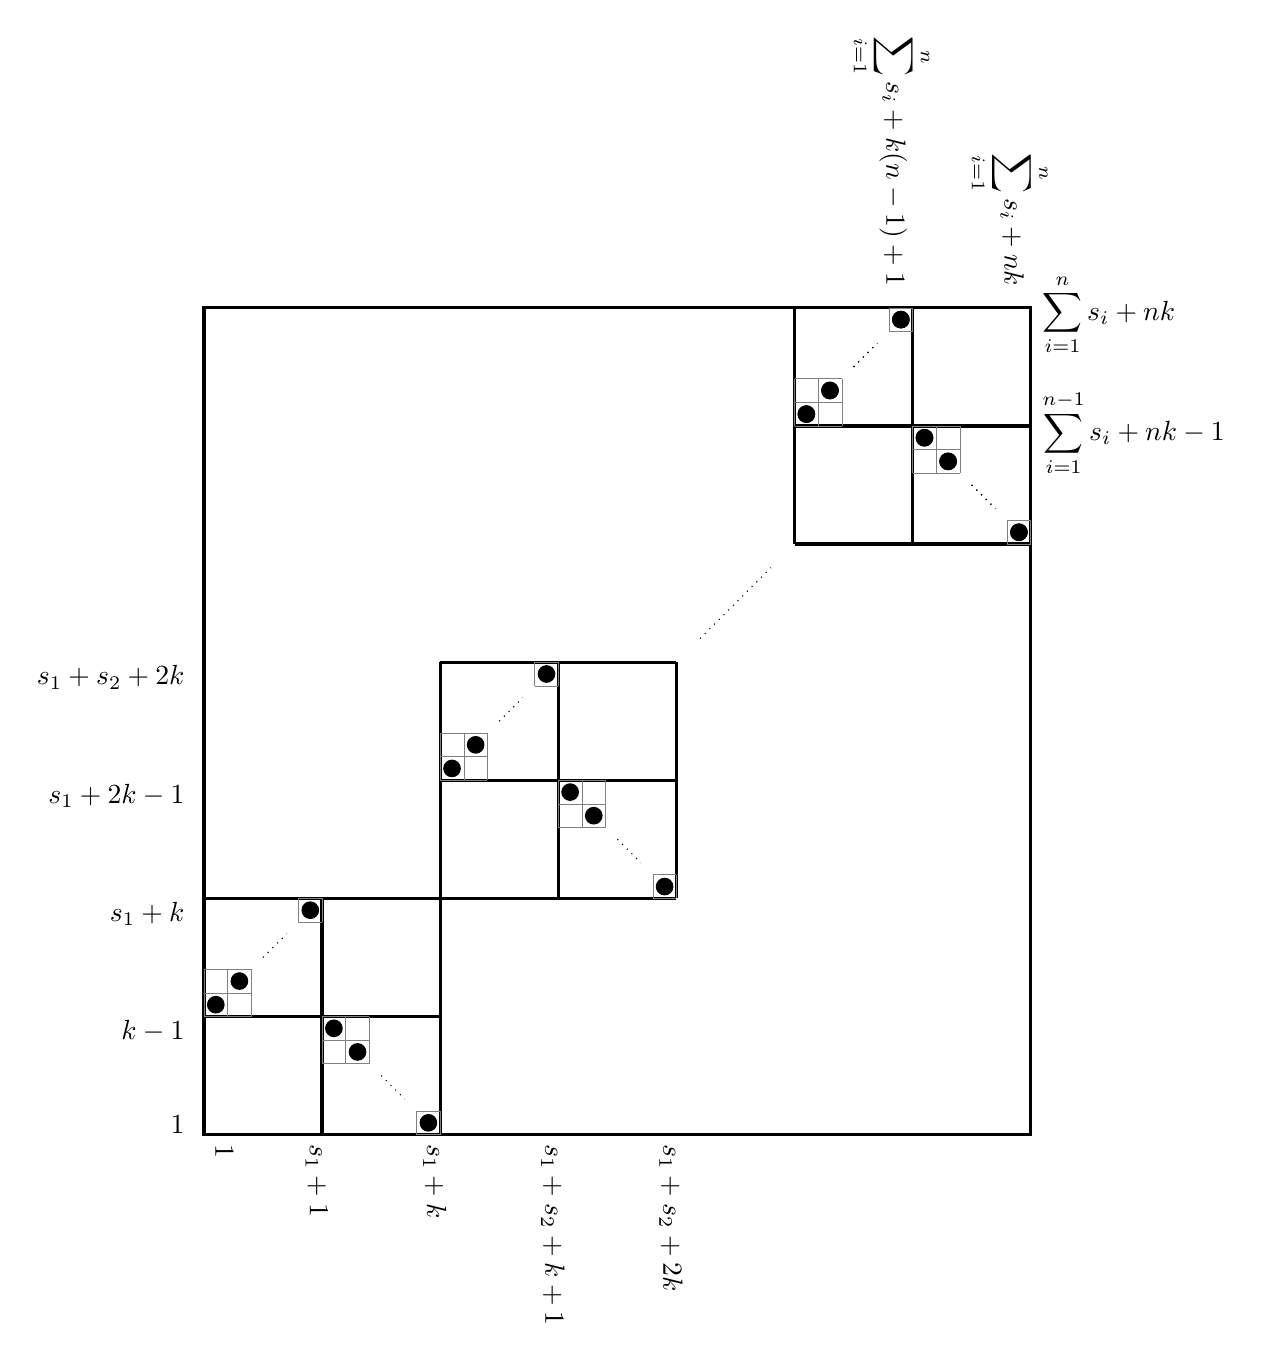
\begin{tikzpicture}
    [
      scale=.3,
    ]
    %
    \draw [black,very thick] (0, 0) rectangle (35, 35);
    \draw [step=5cm,very thick] (0, 0)   grid (10, 10);
    \draw [step=5cm,very thick] (10, 10) grid (20, 20);
    \draw [dotted] (21, 21) -- (24, 24);
    \draw [step=5cm,very thick] (25, 25) grid (35, 35);

    \foreach \x/\y in {0/0, 10/10,25,25} {
      % increasing
      \draw [black, help lines] (\x + 0, \y + 5) grid (\x + 2, \y + 7);
      \draw [black, help lines] (\x + 4, \y + 9) grid (\x + 5, \y + 10);
      \draw [black,fill=black] (\x + 1 - .5, \y + 6 -.5) circle (0.35);
      \draw [black,fill=black] (\x + 2 - .5, \y + 7 -.5) circle (0.35);
      \draw [dotted] (\x + 2.5, \y + 7.5) -- (\x + 3.5, \y + 8.5);
      \draw [black,fill=black] (\x + 5 - .5, \y + 10 -.5) circle (0.35);

      % decreasing
      \draw [black, help lines] (\x + 5, \y + 3) grid (\x + 7, \y + 5); 
      \draw [black, help lines] (\x + 9, \y + 0) grid (\x + 10, \y + 1);
      \draw [black,fill=black] (\x + 6 - .5, \y + 5 -.5) circle (0.35);
      \draw [black,fill=black] (\x + 7 - .5, \y + 4 -.5) circle (0.35);
      \draw [dotted] (\x + 7.5, \y + 2.5) -- (\x + 8.5, \y + 1.5);
      \draw [black,fill=black] (\x + 10 - .5, \y + 1 -.5) circle (0.35);
    }

    % x-labels
    \node [label={[text depth=1.75ex,label distance=0.0cm,rotate=-90]right:{$1$}}] at (0,0) {};
    \node [label={[text depth=1.75ex,label distance=0.0cm,rotate=-90]right:{$s_1+1$}}] at (4,0) {};
    \node [label={[text depth=1.75ex,label distance=0.0cm,rotate=-90]right:{$s_1+k$}}] at (9,0) {};
    \node [label={[text depth=1.75ex,label distance=0.0cm,rotate=-90]right:{$s_1+s_2+k+1$}}] at (14,0) {};
    \node [label={[text depth=1.75ex,label distance=0.0cm,rotate=-90]right:{$s_1+s_2+2k$}}] at (19,0) {};
    \node [label={[text depth=1.75ex,label distance=0.0cm,rotate=-90,anchor=east]right:{$\displaystyle\sum_{i=1}^{n}s_i+k(n-1)+1$}}] at (29,35.5) {};
    \node [label={[text depth=1.75ex,label distance=0.0cm,rotate=-90,anchor=east]right:{$\displaystyle\sum_{i=1}^{n}s_i+nk$}}] at (34,35.5) {};

    % y labels
    \node [label={[text depth=1.75ex,label distance=0.0cm,anchor=east]left:{$1$}}] at (0, 0) {};
    \node [label={[text depth=1.75ex,label distance=0.0cm,anchor=east]left:{$k-1$}}] at (0, 4) {};
    \node [label={[text depth=1.75ex,label distance=0.0cm,anchor=east]left:{$s_1+k$}}] at (0, 9) {};
    \node [label={[text depth=1.75ex,label distance=0.0cm,anchor=east]left:{$s_1+2k-1$}}] at (0, 14) {};
    \node [label={[text depth=1.75ex,label distance=0.0cm,anchor=east]left:{$s_1+s_2+2k$}}] at (0, 19) {};
    \node [label={[text depth=1.75ex,label distance=0.0cm,anchor=west]left:{$\displaystyle\sum_{i=1}^{n-1}s_i+nk-1$}}] at (35.5, 30) {};
    \node [label={[text depth=1.75ex,label distance=0.0cm,anchor=west]left:{$\displaystyle\sum_{i=1}^{n}s_i+nk$}}] at (35.5,35) {};
  \end{tikzpicture}
  \caption{\label{fig:bin-packing}%
  \textsc{Bin Packing}.}
\end{figure}


  We claim that the $n$ items $s_1, s_2, \dots, s_n$
  can be partitioned into $k$ susbets, each of total size $B$,
  if and only if
  $\pi$ can be colored by $k$ increasing permutations of length $B+n$.

  $(\Rightarrow)$
  Suppose that the $n$ items $s_1, s_2, \dots, s_n$
  can be partitioned into $k$ susbets, each of total size $B$.
  Write $S = S_1 \cup S_2 \cup \dots \cup S_k$ such a partition.
  Define a $k$-coloring of $\pi$ as follows.
  Consider any
  $\left(\mathbf{\nearrow}_{s_i+1} \ominus \mathbf{\searrow}_{k-1}\right)$
  pattern of $\pi$,
  and suppose that $s_i \in S_j$.
  Color the whole ascending pattern $\mathbf{\nearrow}_{s_i+1}$ with color $c_j$
  and color arbitrarily the elements of the descending pattern
  $\mathbf{\searrow}_{k-1}$ with the remaining $k-1$ colors
  (each element of $\mathbf{\searrow}_{k-1}$ is assigning a distinct color).
  We claim that every color $c_j$, $1 \leq j \leq k$, induces an increasing pattern
  of length $B+n$ in $\pi$.
  First, it is clear that the above $k$-coloring induces increasing patterns only.
  As for the length of each induced increasing pattern, focus on any color
  $c_j$, $1 \leq j \leq k$.
  We note that in every
  $\left(\mathbf{\nearrow}_{s_i+1} \ominus \mathbf{\searrow}_{k-1}\right)$
  pattern of $\pi$, either the whole $\mathbf{\nearrow}_{s_i+1}$ subpattern is
  colored with color $c_j$ (if $s_i \in S_j$) or exactly one element of the
  $\mathbf{\searrow}_{k-1}$ subpattern is colored with color $c_j$
  (if $s_i \notin S_j$).
  Then it follows that the increasing pattern induced by color $c_j$ in $\pi$ has
  length
  $\sum_{s_i \in S_j} \left(s_i + 1\right) + n - |S_i|
  =
  \sum_{s_i \in S_j} s_i + |S_i| + n - |S_i|
  = B + n$.

  $(\Leftarrow)$
  Suppose now that there exists a $k$-coloring of $\pi$ such that each color
  induces
  an increasing pattern of length $B+n$.
  Observe that every
  $\left(\mathbf{\nearrow}_{s_i+1} \ominus \mathbf{\searrow}_{k-1}\right)$
  pattern requires at least $k$ colors as it contains a decreasing subpattern of
  length $k$.
  Therefore the whole $\mathbf{\nearrow}_{s_i+1}$ subpattern is colored with the
  same color.
  For every $1 \leq j \leq k$, define $S_j$ to be the set of all $s_i$ such that
  in the $i$-th
  $\left(\mathbf{\nearrow}_{s_i+1} \ominus \mathbf{\searrow}_{k-1}\right)$
  pattern, the $\mathbf{\nearrow}_{s_i+1}$ subpattern is colored with color $c_j$.
  Therefore, for every $1 \leq j \leq k$, we have
  $B + n = \sum_{s_i \in S_j} \left(s_i+1\right) + n - |S_j|
  = \sum_{s_i \in S_j} s_i + |S_j| + n - |S_j|$,
  and hence
  $\sum_{s_i \in S_j} s_i = B$.
  Therefore, the $n$ items $s_1, s_2, \dots, s_n$
  can be packed into $k$ bins, each of capacity $B$.
\end{proof}
